\subsubsection{Speisung}

Die Speisung ist mehrstufig realisiert. Zum einen gibt es eine Speisung
welche die Energie für die Logikeinheiten liefert. Diese wird per Netzadapter
an das Raspberry Pi geführt. Dieses bildet die High-Level-Logik und somit die
zentrale Einheit welche eine 5 Volt Speisung zur Verfügung stellt an den
USB-Schnittstellen des Einplatinencomputers. Das Raspberry Pi wird per
USB-Kabel mit dem Freedomboard verbunden, über welches nebst den
Datenleitungen auch die Speisung geführt wird. So ist sichergestellt,
dass beide Einheiten eine gemeinsame Speisung haben welche auch der
logischen Hirachie folgt. Das Freedomboard selbst stellt eine weitere
Speisung bereit auf dem eigenen Logikpegel von 3.3 Volt. Die Abbildung
\ref{fig:et-block_logic} zeigt das Blockschaltbild mit ausgeblendeten
Einheiten wleche nicht von der Logikspeisung betrieben werden.

\begin{figure}[h!]
	\centering
	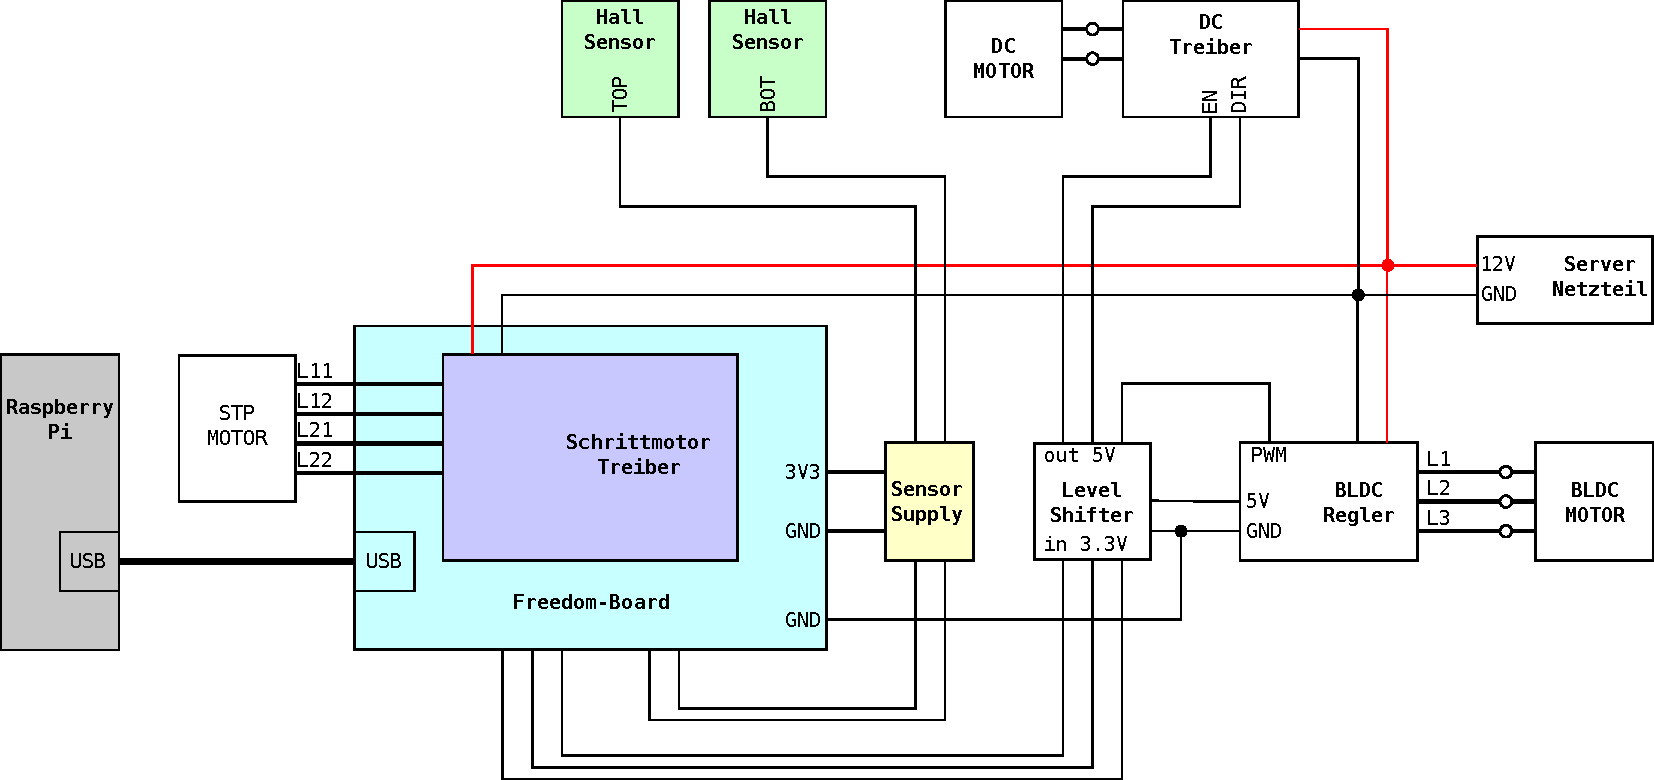
\includegraphics[width=0.95\textwidth]{../../fig/blockdiagram_logic.pdf}
	\caption{Blockschaltbild der Logikspeisung}
	\label{fig:et-block_logic}
\end{figure}

Nebst der Speisung für die Logik, welche auch die Komminukation zwischen
Raspberry Pi und Freedomboard ermöglicht, bedarf es auch einer
Leistungsspeisung. Diese wird mittels eines Servernetzteils zur Verfügung
gestellt. Das Servernetzteil bietet eine 12 Volt Speisung welche für sämtliche
Motoren eingesetzt wird. Auf diese Weise kann eine satte Speisung
gewährleistet werden wleche auch für höhere Leistungsänderungen fähig ist.
Nebst den Motoren und den zugehörigen Treibern wird auch der 3.3 Volt zu 
5 Volt Pegelwandler durch die Leistungsspeisung betrieben. Hierzu wird der
interne 5 Volt Spannungsregler der Brushlessansteuerung genutzt, welcher durch
die Leistungsspeisung betrieben wird. Dies garantiert stabile Pegel für die
Ansteuerung des Brushlessreglers so wie dies im beabsichtigen Einsatz
vorgesehen ist.



